\documentclass[english,serif,mathserif,xcolor=pdftex,dvipsnames,table]{beamer}

\usepackage[T1]{fontenc}
\usepackage[utf8]{inputenc}

\usetheme[informal]{s3it}
\usepackage{s3it}

\title[Introduction to Python]{%
  A Short and Incomplete Introduction to Python
}
\subtitle{\bfseries Part 0: Introduction}
\author[R.~Murri]{%
  Riccardo Murri \texttt{<riccardo.murri@uzh.ch>}
  \\
  S3IT: Services and Support for Science IT,
  \\
  University of Zurich
}
\date{June~8, 2017}


\begin{document}

% title frame
\maketitle

\begin{frame}
  \begin{center}
    {\Huge Welcome!}
  \end{center}
\end{frame}


% \begin{frame}
%   \frametitle{What is S3IT?}

%   \begin{center}
%     {\em ``A partner for data- and \\ compute-intensive science''}

%     \+
%     \begin{description}
%     \item[Enable] researchers and projects to run simulations and data analysis.
%     \item[Develop] tools to integrate, automate and scale scientific use cases.
%     \item[Provide] access to {\em innovative} infrastructures and technologies.
%     \end{description}

%     \+
%     {\em \small{Want to know more? }\url{http://www.s3it.uzh.ch}}
%   \end{center}
% \end{frame}


\begin{frame}
  \frametitle{Prerequisites}
  This course assumes a basic experience with computer programming.

  \+
  Any language should do, as long as you are already familiar with
  the concepts of variables and functions.
\end{frame}


\begin{frame}[fragile]
  \frametitle{Python 2 \emph{vs} Python 3}

  There are currently two major versions of Python available, with
  slightly different syntax and features.

  \+
  Python 2.7 is the last release in the 2.x series.

  \+
  Python 3.x has a more polished syntax, removing inconsistencies and
  some historical baggage.

  \+
  In this course we will focus on \textbf{Py3 syntax}.
  % But Python 2.x is still the default on most Linux distributions, so
  % \textbf{we shall focus on Py2 syntax}.

  \+
  {\footnotesize\em
    Watch a debate between ``Pro'' and ``Contra'' advocates:
    \url{http://www.physik.uzh.ch/~nchiapol/webm/3_1_Python3.webm}}

  \+
  {\footnotesize\em
    Explore the key differences:
    \url{http://tinyurl.com/py2-and-py3-key-differences}}
\end{frame}


\begin{frame}
  \frametitle{Talk outline}
  \begin{enumerate}
  \item Python basics
  \item NumPy and plotting
  %\item Pandas and how to query tabular data
  \item Workflows with GC3Pie
  \end{enumerate}
\end{frame}


\begin{frame}
  \frametitle{Next steps}

  The course will be structured as a mixture of slides and hands-on
  sessions for practicing Python programming.

  \+
  So, the very first step is making sure you can access the Jupyter/IPython
  server for running the exercise notebooks.
\end{frame}


\part{How to run Python code}

\begin{frame}[fragile]
  \frametitle{The Python shell, I}
  Python is an \emph{interpreted} language.

  \+
  It also features an interactive
  \href{http://en.wikipedia.org/wiki/REPL}{``shell''} for evaluating
  expressions and statements immediately.

  \+
  The IPython shell is started by invoking the command
  \texttt{ipython} in a terminal window.
\begin{semiverbatim}\tiny
\$ \textbf{ipython}
Python 2.7.13 |Anaconda 4.3.0 (64-bit)| (default, Dec 20 2016, 23:09:15)
Type "copyright", "credits" or "license" for more information.

IPython 5.1.0 -- An enhanced Interactive Python.
?         -> Introduction and overview of IPython's features.
%quickref -> Quick reference.
help      -> Python's own help system.
object?   -> Details about 'object', use 'object??' for extra details.

\textbf{In [1]:}{\color{blue}\normalfont\em \(\leftarrow\) here is where you enter commands}
\end{semiverbatim}
\end{frame}


\begin{frame}
  \frametitle{The IPython notebook, I}

  \begin{columns}[t]
    \begin{column}{0.5\textwidth}
      \begin{center}
        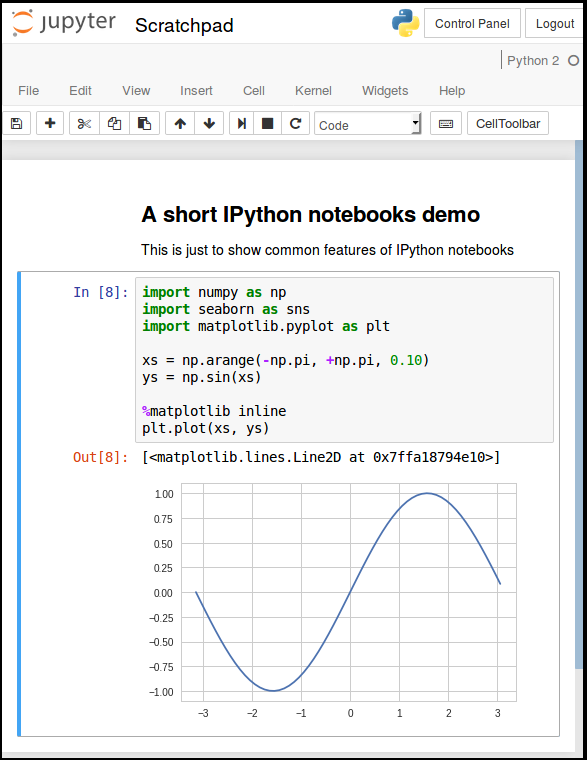
\includegraphics[width=1.00\linewidth]{fig/nb.png}
      \end{center}
    \end{column}
    \begin{column}{0.5\textwidth}
      \small

      A more appealing way of interacting with Python is through the IPython
      notebooks.

      \+
      Notebooks are made of ``cells'', which come in two flavors:
      \begin{itemize}
      \item documentation cells, containing text formatted according to the
        \href{http://commonmark.org/help/}{Markdown} conventions;
      \item code cells, containing arbitrary Python code
      \end{itemize}
    \end{column}
  \end{columns}
\end{frame}


\begin{frame}
  \frametitle{The IPython notebook, II}

  To run Python code in the notebook:
  \begin{itemize}
  \item Type your code in a cell besides the {\ttfamily\bfseries\color{blue}
      In~[~]:} (multiple lines are allowed)
  \item Press \textbf{Ctrl+Enter} to evaluate the cell (prompt changes to
    {\ttfamily\bfseries\color{blue} In~[*]:}) --- or press \textbf{Alt+Enter} to
    evaluate the code \emph{and} open a new code cell.
  \item When the Python kernel has done computing, the result appears \emph{under} the
    code cell marked with a {\ttfamily\bfseries\color{red} Out~[~]:} label.
  \end{itemize}

\end{frame}


\begin{frame}[fragile,fragile]
  \frametitle{The Python shell, II}
  \smaller

  Expressions can be entered at the Python shell prompt; they are evaluated and the
  result is printed:
\begin{semiverbatim}
\In 2+2
\Out 4
\end{semiverbatim}

  \+ Note that the classic Python shell uses `\texttt{>{}>{}>}' as a prompt;
  expression evaluation works exactly the same, though:
\begin{semiverbatim}
>{}>{}> 2+2
4
\end{semiverbatim}

  \+ Throughout these slides, all Python code marked with either `{\color{blue}
    In~[*]}' or `\texttt{>{}>{}>}' can also be entered and evaluated in the IPython
  notebook cells.
\end{frame}


\end{document}

%%% Local Variables:
%%% mode: latex
%%% TeX-master: t
%%% End:
